\documentclass[12pt, titlepage]{article}

\usepackage{hyperref}
\usepackage{graphicx}
\graphicspath{{../.Provided resources/}}
\usepackage{wrapfig} % allows us to create the figures with wrapping text
\usepackage{blindtext}

\title{Including Images}
\author{Me}
\date{\today}

\begin{document}
\maketitle

\newpage
\tableofcontents
\newpage

\section{Including Images}
% \includegraphics[scale = 0.29]{../.Provided resources/plot.jpg}
\includegraphics[width = 0.5\textwidth]{plot.jpg}

\section{Figure env}
This env is similar to the table env
\begin{figure}[h]
    \centering
    \caption{This is a nice plot.}
    \includegraphics[width = 0.5\textwidth]{plot.jpg}
    \caption{This is a nice plot.}
\end{figure}

\newpage
\listoffigures
\listoftables

\section{Figures Wrapped in Text}
\begin{wrapfigure}{l}{0.5\textwidth} % allign left / right and specify the width of the img
    \includegraphics[width = 0.5\textwidth]{plot.jpg}
    \caption{This is a nice plot.}
\end{wrapfigure}
\blindtext

\newpage
\section{Exercise: Including Images}
Pretty tedious... I already played with this env.

\end{document}